\documentclass[11pt,UTF8]{ctexart}
\usepackage{enumerate}
\usepackage{amsmath}
\usepackage{geometry}
\usepackage{booktabs}
\usepackage{textcomp}
\usepackage{mhchem}
\usepackage{graphics}
\usepackage{graphicx} %插入图片的宏包
\usepackage{float} %设置图片浮动位置的宏包
\usepackage{subfigure} %插入多图时用子图显示的宏包
\usepackage[]{caption2}
\geometry{a4paper, left=1.5cm, top=2cm, right=1.5cm, bottom=2cm}
\usepackage{indentfirst}
%\renewcommand{\figurename}{\textbf{图}} %重定义编号前缀词
%\renewcommand{\captionlabeldelim}{\textbf{.~}} 
\newenvironment{unicaption}{\noindent\small}{\normalsize}
\providecommand{\keywords}[1] {
    \textbf{\heiti{关键词\quad{}\kaishu}} #1
}
\providecommand{\enkeywords}[1] {
    \textbf{Keywords\quad{}} #1
}
\CTEXsetup[format={\Large\bfseries\heiti}]{section}
\CTEXsetup[format={\large\bfseries\heiti}]{subsection}
\CTEXsetup[format={\kaishu}]{subsubsection}
\ctexset{abstractname = \heiti{摘\quad{}要}}
% \pagestyle{plain}
% \geometry{left=1.0cm,right=1.0cm,top=1.0cm,bottom=2.0cm}
\title{\textbf{\Large 双光束分光光度计结构分析及其在胰蛋白酶动力学分析中的应用}}
\author{\fangsong 朱嘉悦 2000012267(组长),朱瑾煜 2000012180(安全员) \\ 
        \fangsong 杨霄翔 2000012130,王欣雨 2000012108,李晨暄 2000012273 \\
        \small{\kaishu(北京大学生命科学学院,北京 100871)}}
\date{}

\begin{document}
    \maketitle
    \begin{abstract}
        \kaishu
        分光光度计(spectrophotometer)是定量测定溶液吸光度的仪器,在生物化学实验中的物质浓度测定、酶动力学分析等方面有重要的用途。常用的双光束紫外-可见分光光度计将光束一分为二,省去了调零的步骤。胰蛋白酶(trypsin)是广泛存在于脊椎动物中的一种消化酶,其专一性地将蛋白质水解为短肽,是酶学研究的经典材料和生物学实验中常用的工具酶。本文中,作者分析一款双光束分光光度计的光学结构,以此阐明其测量吸光度及溶液浓度的原理,并使用该分光光度计测定商品胰蛋白酶的酶活力、比活力、米氏常数(\(K_\mathrm{m}\))及抑制剂苯甲脒对胰蛋白酶的抑制效应。

        \keywords{双光束分光光度计;胰蛋白酶;酶动力学;酶活力;米氏常数}
    \end{abstract}
    \renewcommand{\abstractname}{Abstract}

    \begin{center}
        \textbf{\Large Structural analysis of the double beam spectrophotometer \\ and its application on kinetic analysis of trypsin}
        
        \normalsize ZHU Jiayue, ZHU Jinyu, YANG Xiaoxiang, WANG Xinyu, LI Chenxuan

        \small{(\textit{School of Life Sciences, Peking University, Beijing 100817})}
    \end{center}

    \maketitle
    \begin{abstract}
        Spectrophotometer is an instrument for quantitative determination of solution absorbance, which has important applications on determination of concentration and enzyme kinetic analysis in biochemical experiments. A commonly used double beam UV-Vis spectrophotometer splits the beam in two, thus eliminating the step of zero adjustment. Trypsin is a digestive enzyme widely occuring in vertebrates, specifically hydrolyzing proteins into small peptides. It is a classical material in enzymology research and a common tool enzyme in biological experiments. In this paper, the authors analyze the optical structure of a double beam spectrophotometer, in order to reveal the principle of measuring absorbance and solution concentration, and apply the spectrophotometer to determine the enzyme activity, specific activity, Michaelis constant (\(K_\mathrm{m}\)) of commercial trypsin and the inhibitory effect of inhibitor benzamidine on trypsin.

        \enkeywords{Double beam spectrophotometer; Trypsin; Enzyme kinetics; Enzyme activity; Michaelis constant}
    \end{abstract}

    

    \section{材料与方法}
    \subsection{主要仪器}
    本文中涉及的大型仪器主要包括双光束紫外-可见分光光度计、酶标仪、电泳仪、pH 计和水浴锅。

    其中,双光束紫外-可见分光光度计用于本文中大部分的吸光度测量;酶标仪用于 Bradford 法测定胰蛋白酶浓度;电泳仪用于 SDS-PAGE 测定胰蛋白酶的相对分子质量;pH 计用于测定溶液 pH;水浴锅用于研究不同温度条件下的胰蛋白酶活力时的温度调节。

    \subsection{试剂与材料}
    化学试剂均为分析纯。固体商品胰蛋白酶为 Solarbio 公司生产;两种液体商品胰蛋白酶为 gibco 公司生产,其中一种为常温保存,另一种为 \(-20\ \textcelsius\) 保存。为简便起见,本文中将这三种商品胰蛋白酶分别称为固体胰蛋白酶、常温液体胰蛋白酶、冻存液体胰蛋白酶。

    \subsection{SDS-PAGE 测定胰蛋白酶的相对分子质量}
    使用十二烷基硫酸钠聚丙烯酰胺凝胶电泳(sodium dodecyl sulfate polyacrylamide gel electrophoresis, SDS-PAGE)的方法测定商品胰蛋白酶的相对分子质量。
    
    实验中一共进行了两次 SDS-PAGE。首先对样品进行稀释,金属浴加热后离心;然后组装凝胶模,制备分离胶灌入凝胶模中,去离子水密封,待分离胶完全聚合,倒出去离子水,制备并灌入浓缩胶;之后将凝胶板安装在电泳槽中,加电极缓冲液,上样并开始电泳。电泳结束后,取出凝胶,去除浓缩胶,放入已装有25 mL染色液的容器中,完成染色、脱色和照相。

    第二次 SDS-PAGE 的样品制备和上样方案如表 1、表 2 所示。第二次 SDS-PAGE 的样品制备和上样方案见补充表 1、补充表 2。

    \subsection{Bradford 法测定胰蛋白酶浓度}
    在预实验中,根据标准曲线的吸光度,已经确定在使用 Bradford 法测量蛋白浓度时,固体胰蛋白酶的浓度在 \(10\ \mathrm{mg/mL} \sim 40\ \mathrm{mg/mL}\) 为宜,\(-20\ \textcelsius\) 保存的液体胰蛋白酶浓度在 \(0.5\ \mathrm{mg/mL} \sim 1.5\ \mathrm{mg/mL}\) 为宜。对于常温液体胰蛋白酶,即使把原来的 \(\mathrm{5\ \mu L}\) 上样体积变为 \(\mathrm{20\ \mu L}\),其吸光度依然低于上样量为 \(\mathrm{4\ \mu L}\) 的 BSA 标准蛋白溶液。因此,常温液体胰蛋白酶不适宜后续实验。

    正式实验中,按照如表 3 所示的加样体积及测定步骤,使用 Bradford 法,在酶标仪中、595 nm 下,测出每组溶液的吸光度。在此之后,在固体胰蛋白酶和冻存液体胰蛋白酶的多个浓度中,选择一组较好的数据进行分析,估算出原溶液中的蛋白质浓度。

    \subsection{胰蛋白酶活力测定方法}
    \subsubsection{配置底物溶液}
    每 50 mL 底物混合溶液中含 0.5 mL 2 mol/L \(\ce{CaCl2}\)溶液,0.5 mL \(\mathrm{pH=8.0}\) 2 mol/L 底物 BAEE 溶液,其余体积用 0.1 mol/L Tris-HCl (Base)、0.1 mol/L HCl 溶液和超纯水混合并调 pH,定容至 50 mL。共配制 \(\mathrm{pH = 5.00, 6.00, 6.95, 7.19, 7.68, 7.85, 8.05, 8.26, 8.53, 9.03, 9.45}\) 等 11 种 pH 梯度的底物溶液。
    \subsubsection{底物溶液的水浴保温处理}
    使用恒温金属浴加热 \(\mathrm{pH=8.05}\) 的底物溶液。除常温一组外,底物溶液分别加热到 45 \textcelsius、60 \textcelsius、70 \textcelsius、80 \textcelsius、95 \textcelsius。每个温度设置两个 1.5 mL 离心管进行加热,加热时间为 10 分钟。
    \subsubsection{加样}
    测定 pH 对酶活力影响时,对三种胰蛋白酶分别测定。将底物溶液和酶溶液(实验组)或 \(\mathrm{pH=3\ HCl}\)溶液加入比色皿中。酶溶液均用 \(\mathrm{pH=3\ HCl}\)溶液 配制或稀释。具体加样量如表 4 所示。

    测定温度对酶活力影响时,选择冻存液体胰蛋白酶进行测定。加样量同表 4,但考虑到高温对化学反应的促进作用,使用的是稀释至 \(0.02 \times\) 的酶溶液。
    \subsubsection{酶活力测定}
    使用双光束紫外-可见分光光度计的动力学模式,在加入酶溶液的同时开始测量 \(A_\mathrm{253\ nm}\),每 6 s 或 15 s 测量一组数据,测量时间为 90 s。测量结果绘制成 \(A_\mathrm{253\ nm}\) 对时间的图象,并拟合出曲线,求得原点附近的切线斜率 \(\Delta A = \mathrm{d}A_\mathrm{253\ nm}/\mathrm{d}t\)。根据公式 (1)
    \begin{equation}
        \mathrm{Enzyme activity} = \frac{\Delta A\cdot V}{\epsilon L},
    \end{equation}
    其中 \(V\) 为比色皿中液体的体积,\(epsilon\) 为底物 BAEE 的摩尔吸光系数(取文献值 600 L/mmol·cm),\(L\) 为比色杯的光程(1 cm)。\(\Delta A\) 的具体计算方法参见 1.8 节。

    \subsection{胰蛋白酶的米氏常数(\(K_\mathrm{m}\))测定方法}
    取 12 支试管,分别编号 \(1 \sim 12\)。完毕后,按照表 5 中的加样体系加样。

    反应完毕后,分别在双光束分光光度计中测量试管中溶液的 410 nm 处吸光值,并根据公式 (2)
    \begin{equation}
        v=\frac{A_\mathrm{410\ nm}}{8\ 800\times 10^{-3}\times 60\times 2}
    \end{equation}    
    计算出酶的反应速率。完毕后,以\(\mathrm{[S]/v}\)为纵坐标,底物浓度\(\mathrm{[S]}\)为横坐标,用 Hanes 法作图。

    \subsection{胰蛋白酶抑制剂的抑制效应测定方法}
    

    \subsection{数据处理、图表绘制及统计分析方法}
    本实验中的数据处理、图表绘制及统计分析主要使用 R 语言(版本号 4.2.0)完成。使用的宏包主要包括 \texttt{ggplot2} 和 \texttt{tidyverse}。运行的操作系统为 macOS Monsterey 12.3.1。

    处理测量酶活力的吸光度与时间的数据时,使用 R 语言的 \texttt{ggplot2} 包,通过局部加权回归(locally weighted regression, LOESS),作出平滑的时间-吸光度平滑曲线。计算 \(\Delta A\) 时,传统的方法是在原点作切线,然后直接在图中读出 1 min 时的吸光度大小。这种方法误差较大,我们不妨直接通过拟合曲线在原点左右的数据来计算。注意到该曲线是通过 LOESS 拟合的,实际上是通过很多段小的直线线段拼接而成的,因此只需要取原点附近的一小段直线线段,以其斜率作为 \(\Delta A\)。为了减小误差,我们取原点附近的 4 个作图点 \(P_1, P_2, P_3, P_4\),取 \(P_1P_2\) 与 \(P_3P_4\) 斜率的平均值作为 \(\Delta A\)。LOESS 拟合后的作图数据通过 \texttt{ggplot\_build()} 函数很容易得到。

    \section{结果}
    \subsection{双光束分光光度计的结构分析}
    对老式双光束紫外-可见分光光度计进行拆卸,具体过程如补充图 1 所示。拆卸后的分光光度计内部结构及其光路示意如图 1 所示。
    
    \begin{figure}[H] %H为当前位置,!htb为忽略美学标准,htbp为浮动图形
        \centering %图片居中
        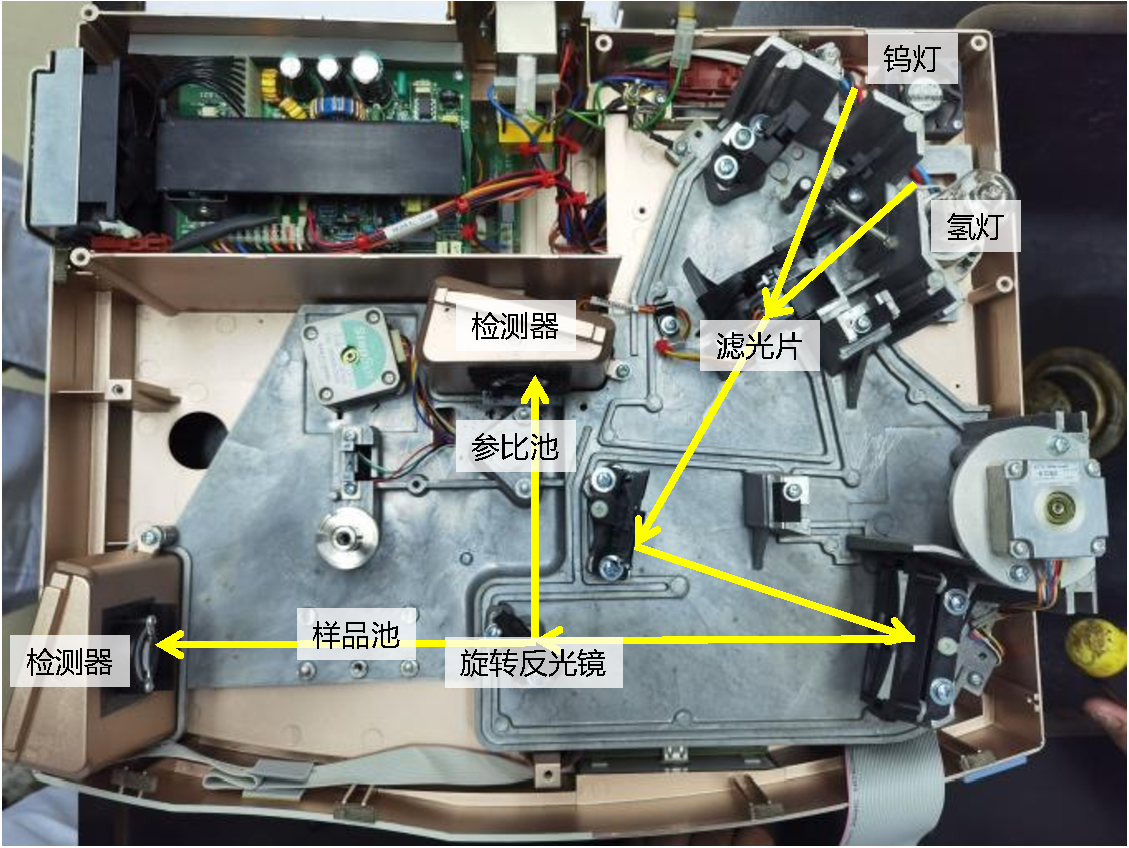
\includegraphics[width=0.7\textwidth]{optical.pdf} %插入图片,[]中设置图片大小,{}中是图片文件名
        %\caption{分光光度计内部结构及其光路示意} %最终文档中希望显示的图片标题
        %\label{图 1. 分光光度计内部结构及其光路示意} %用于文内引用的标签
    \end{figure}

    \begin{unicaption}
        \textbf{图 1. 老式双光束紫外-可见分光光度计内部结构及其光路示意。}图中用文字标明各内部结构的名称,用黄色箭头表示光路。光从钨灯(可见光)或氢灯(紫外光)发出,经狭缝进入滤光片,成为指定波长的单色光;单色光进而经过旋转反光镜的反射和透射,分别射入参比池和样品池,并被各自的检测器检测吸光度。
    \end{unicaption}

    \subsection{胰蛋白酶的相对分子质量}
        \subsubsection{SDS-PAGE 结果}
        SDS-PAGE 结果显示,除 PM 外仅在 lane 3,即上样量为 \(\mathrm{10\ \mu g}\) 的冻存液体胰蛋白酶有较不明显的两条浅蓝色条带出现,其余泳道无条带出现,如图 2 所示。在此之前,作者还进行了一次 SDS-PAGE 实验,该次实验并未出现可分辨的条带(见补充图 2),可能是因为上样量太少导致(见补充表 1、补充表 2)。

        我们假设图 2 中 lane 3 的两条条带是胰酶的条带进行下述分析,但不排除其不是胰酶条带的可能。

        \subsubsection{标准曲线的制作}
        我们已知对于蛋白质的相对分子质量和电泳迁移率有如公式 (3) 所示的关系:
        \begin{equation}
            \lg{M_\mathrm{r}} = -bm_\mathrm{R} + K,
        \end{equation}

        其中,\(M_\mathrm{r}\)为蛋白质的相对分子质量,\(m_\mathrm{R}\) 为电泳相对迁移率,\(b\) 为斜率,\(K\) 为截距。一般情况下,\(b, K\) 为常数。
        
        故使用 Photoshop 软件测量条带移动距离,所得数据如表 6 所示。根据表 6 可做出标准曲线如图 3。

        
        
        对标准曲线进行拟合得到迁移距离 \(y\) (单位:px)与蛋白质相对分子质量 \(m_\mathrm{R}\) (单位:kDa)的关系为
        \begin{equation}
            y = -747.73\lg{M_\mathrm{r}}+ 1595.7.
        \end{equation}

        \subsubsection{相对分子质量的计算}
        测量冻存液体胰蛋白酶的两个条带移动距离 \(y_1, y_2\),得\(y_1 = 243.00\ \mathrm{px}, y_2 = 570.00\ \mathrm{px}\),将其代入公式 (4) 可得
        \begin{equation}
            M_\mathrm{r1} = 64.29\ \mathrm{kDa}, \quad M_\mathrm{r2} = 23.49\ \mathrm{kDa}.
        \end{equation}
    
    \subsection{固体及冻存液体胰蛋白酶的浓度及纯度}
        使用 Bradford 法测定固体胰蛋白酶和冻存液体胰蛋白酶的浓度,在酶标仪测得吸光度 \(A_\mathrm{595\ nm}\)的结果如表 7 所示。

        按照表 7 数据绘制标准曲线。孔2的标准蛋白质溶液含量为 \(\mathrm{200\ \mu g/mL \times 4\ \mu L =0.8\ \mu g}\),同理可计算得孔号1、2、3、4、5、6的蛋白含量依次为\(\mathrm{0, 0.8\ \mu g, 1.6\ \mu g, 2.4\ \mu g, 3.2\ \mu g, 4.0\ \mu g}\)。由此作出的标准曲线如图 4 所示。

        \begin{unicaption}
            \textbf{表 7. Bradford法测量胰蛋白酶浓度测定结果。} 单位:\(\mathrm{\mu mol/min}\)。
        \end{unicaption}

        \small
        \begin{center}
        \begin{tabular}{cccc}
            \centering
            \toprule  %添加表格头部粗线
            孔号 & 1 & 2 & 3 & 4 & 5 & 6 & 固体胰酶 & 常温液体胰酶 & 冻存液体胰酶 \\
            \midrule  %添加表格中横线
            \(A_\mathrm{595\ nm(1)}\) & 0.520 & 0.866 & 1.022 & 1.175 & 1.293 & 1.445 & 1.163/0.954/0.807 & — & 1.361/1.197/0.972
            \(A_\mathrm{595\ nm(2)}\) & 0.518 & 0.799 & 1.006 & 1.149 & 1.339 & 1.425 & 1.224/0.981/0.800 & — & 1.376/1.228/0.969
            \(A_\mathrm{595\ nm(mean)}\) & 0.519  & 0.833  & 1.014  & 1.162  & 1.316  & 1.435  & 1.194/0.968/0.804 & — & 1.369/1.212/0.971
            \bottomrule %添加表格底部粗线
        \end{tabular}
        \end{center}
        \normalsize

        \begin{figure}[H] %H为当前位置,!htb为忽略美学标准,htbp为浮动图形
            \centering %图片居中
            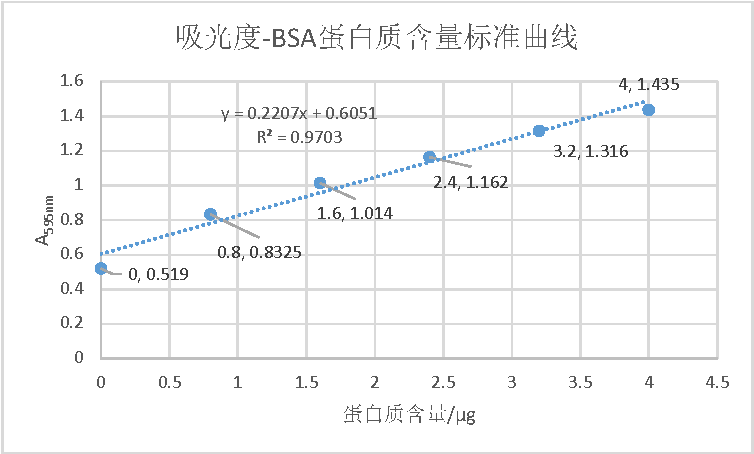
\includegraphics[width=0.7\textwidth]{stdc.pdf} %插入图片,[]中设置图片大小,{}中是图片文件名
            %\caption{分光光度计内部结构及其光路示意} %最终文档中希望显示的图片标题
            %\label{图 1. 分光光度计内部结构及其光路示意} %用于文内引用的标签
        \end{figure}
    
        \begin{unicaption}
            \textbf{图 8. 三种胰蛋白酶在不同pH条件下的吸光度-时间酶动力学曲线。} Solid: 固体胰蛋白酶;Liquid 1: 常温液体胰蛋白酶;Liquid 2: 冻存液体胰蛋白酶。
        \end{unicaption}

        根据标准曲线方程
        \begin{equation}
            y = 0.2207x + 0.6051,
        \end{equation}
        利用测得的样品吸光值 \(y\),可以反推出样品中的蛋白质含量 \(x\),从而计算出2种胰蛋白酶样品的蛋白质浓度,如表 8 所示。


    \subsection{三种胰蛋白酶在不同pH条件下的活力}
        按前述方法,分别测定三种胰蛋白酶在 \(\mathrm{pH = 5.00, 6.00, 6.95, 7.19, 7.68, 7.85, 8.05, 8.26, 8.53, 9.03, 9.45}\) 的酶活力,所得吸光度与时间关系的原始数据见补充表 3,图象如图 5 所示。

        \begin{figure}[H] %H为当前位置,!htb为忽略美学标准,htbp为浮动图形
            \centering %图片居中
            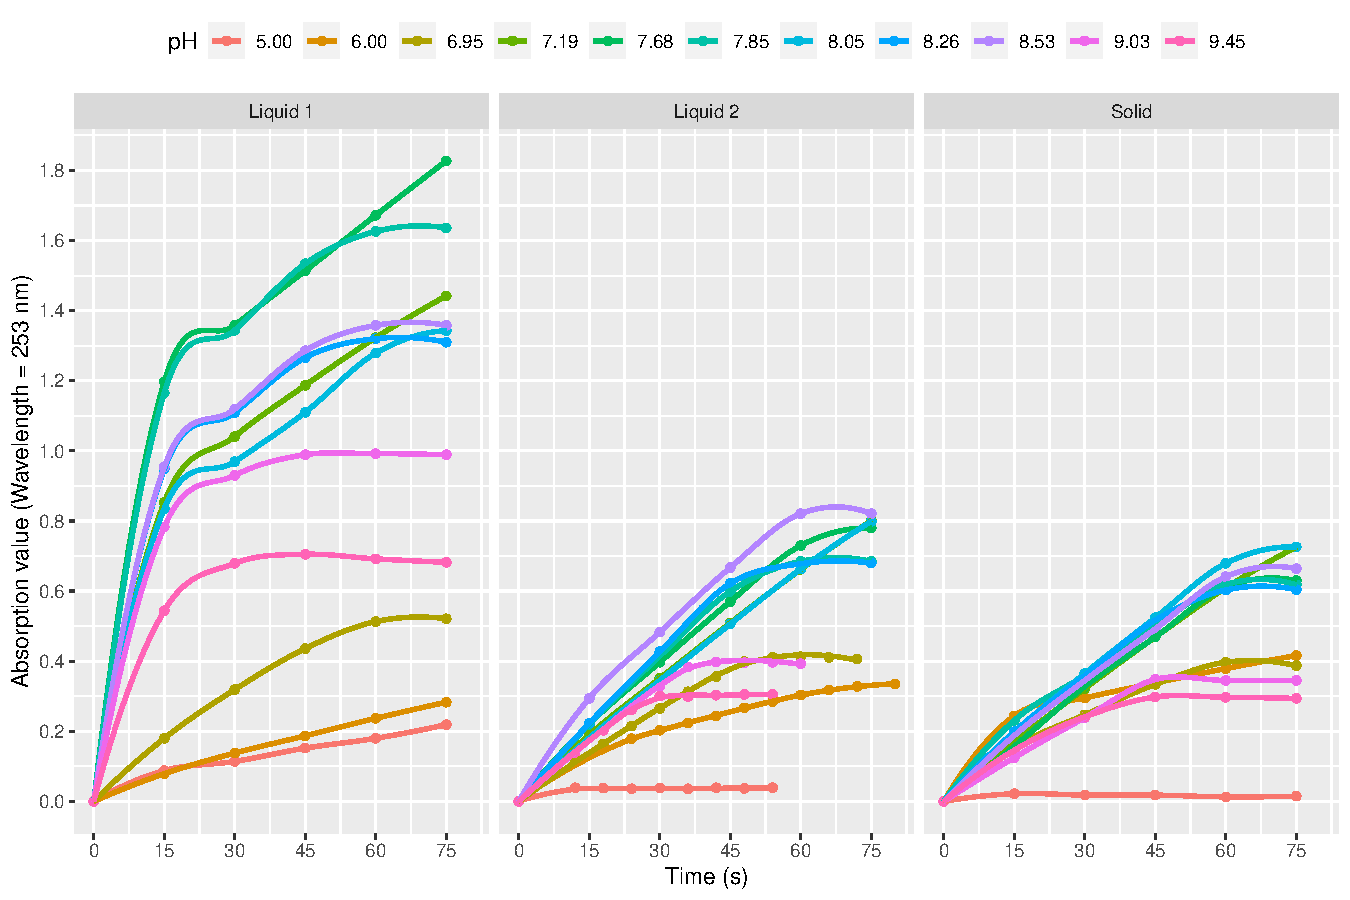
\includegraphics[width=1.0\textwidth]{pH_plot_2.pdf} %插入图片,[]中设置图片大小,{}中是图片文件名
            %\caption{分光光度计内部结构及其光路示意} %最终文档中希望显示的图片标题
            %\label{图 1. 分光光度计内部结构及其光路示意} %用于文内引用的标签
        \end{figure}
    
        \begin{unicaption}
            \textbf{图 5. 三种胰蛋白酶在不同pH条件下的吸光度-时间酶动力学曲线。} Solid: 固体胰蛋白酶;Liquid 1: 常温液体胰蛋白酶;Liquid 2: 冻存液体胰蛋白酶。
        \end{unicaption}

        按 1.8 中方法处理数据,计算出三种胰蛋白酶在不同pH条件下的酶活力,如表 9 所示。

        \begin{unicaption}
            \textbf{表 9. 三种胰蛋白酶在不同pH条件下的酶活力。} 单位:\(\mathrm{\mu mol/min}\)。
        \end{unicaption}

        \small
        \begin{center}
        \begin{tabular}{cccc}
            \centering
            \toprule  %添加表格头部粗线
            pH& 固体胰蛋白酶活力 & 常温液体胰蛋白酶活力 & 冻存液体胰蛋白酶活力 \\
            \midrule  %添加表格中横线
            5 & 0.002413097 & 0.001219113 & 0.000650633 \\
            6 & 0.00185816 & 0.002790232 & 0.006443544 \\
            6.95 & 0.004194295 & 0.002866311 & 0.00361038 \\
            7.19 & 0.023943831 & 0.004034937 & 0.00350962 \\
            7.68 & 0.034488439 & 0.004784557 & 0.003026582 \\
            7.85 & 0.033373705 & 0.004602532 & 0.005446329 \\
            8.05 & 0.02387092 & 0.003757722 & 0.004174937 \\
            8.26 & 0.027024743 & 0.004613924 & 0.004295949 \\
            8.53 & 0.027170025 & 0.006730633 & 0.004011139 \\
            9.03 & 0.022199899 & 0.003620616 & 0.002589114 \\
            9.45 & 0.015139646 & 0.003781534 & 0.003333165 \\
            \bottomrule %添加表格底部粗线
        \end{tabular}
        \end{center}
        \normalsize

    \subsection{冻存液体胰蛋白酶在不同温度条件下的活力}
    按前述方法,测定冻存液体胰蛋白酶在 45 \textcelsius、60 \textcelsius、70 \textcelsius、80 \textcelsius、95 \textcelsius 的酶活力,所得吸光度与时间关系的原始数据见补充表 4,图象如图 6 所示。

    \begin{figure}[H] %H为当前位置,!htb为忽略美学标准,htbp为浮动图形
        \centering %图片居中
        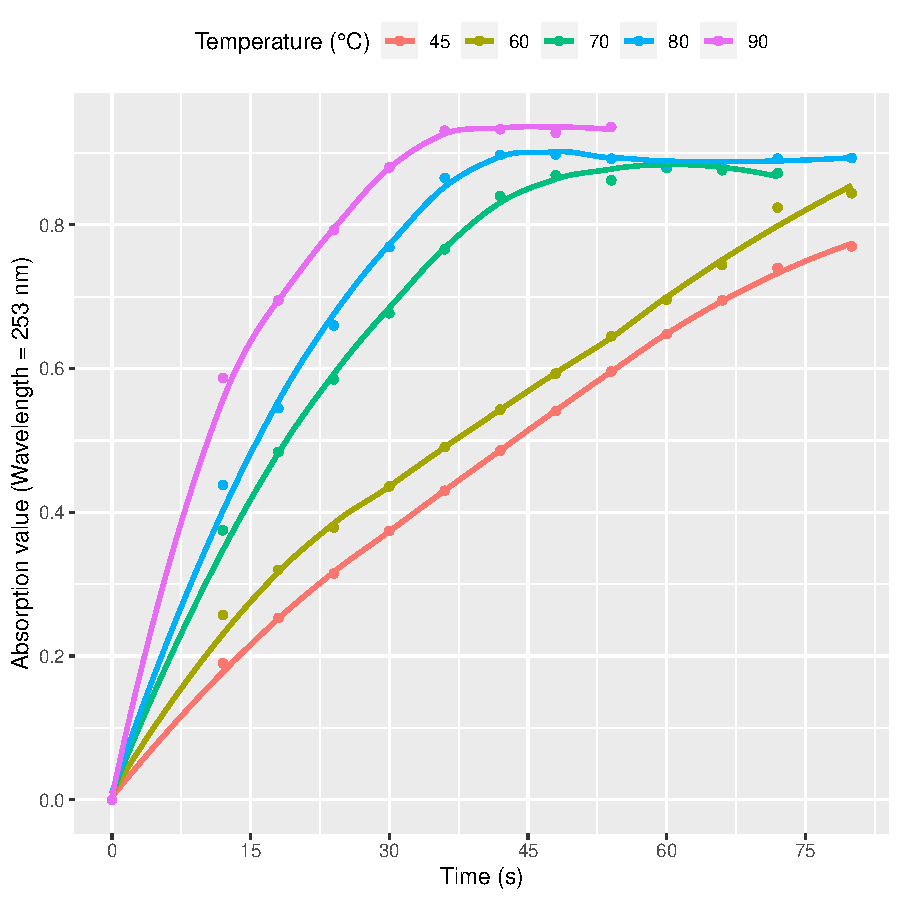
\includegraphics[width=1.0\textwidth]{temp_plot_2.pdf} %插入图片,[]中设置图片大小,{}中是图片文件名
        %\caption{分光光度计内部结构及其光路示意} %最终文档中希望显示的图片标题
        %\label{图 1. 分光光度计内部结构及其光路示意} %用于文内引用的标签
    \end{figure}

    \begin{unicaption}
        \textbf{图 6. 冻存液体胰蛋白酶在不同温度条件下的吸光度-时间酶动力学曲线。} 
    \end{unicaption}

    按 1.8 中方法处理数据,计算出冻存液体胰蛋白酶在不同温度条件下的酶活力,如表 10 所示。

    \begin{unicaption}
        \textbf{表 10. 冻存液体胰蛋白酶在不同温度条件下的酶活力。} 单位:\(\mathrm{\mu mol/min}\)。
    \end{unicaption}

    \small
    \begin{center}
    \begin{tabular}{cc}
        \toprule  %添加表格头部粗线
        温度(\textcelsius)& 冻存液体胰蛋白酶活力 \\
        \midrule  %添加表格中横线
        45	&	0.004654688 \\
        60	&	0.006148615 \\
        70	&	0.009343735 \\
        80	&	0.010883417 \\
        95	&	0.017191829 \\
        \bottomrule %添加表格底部粗线
    \end{tabular}
    \end{center}
    \normalsize

    由图 5、表 9,三种酶的最适 pH 分别为 7.68, 7.68, 7.85。胰蛋白酶的最适 pH 在\(7.5\sim 8.5\)之间。

    \subsection{冻存液体胰蛋白酶的米氏常数(\(K_\mathrm{m}\))分析}
    Hanes 法作图的数据与图如表 11、图 7 所示。

    由米氏方程变型,可知有
    \begin{equation}
        \frac{\mathrm{[S]}}{v}=\frac{K_\mathrm{m}}{V_\max}+\frac{\mathrm{[S]}}{V_\max}.
    \end{equation}
    由标准曲线
    \begin{equation}
        y = 272.61x + 750.92.
    \end{equation}
    可知,本次实验测得的胰蛋白酶动力学参数为:
    \begin{equation}
        V\_max = 1/272.61 = 0.00367\ \mathrm{(mmol/L/sec)}, \quad K_\mathrm{m} = 750.92\times 0.00367 = 2.755\ \mathrm{(mmol/L)}
    \end{equation}

    由图 6、表 10 可见,胰蛋白酶的酶活力随缓冲液温度的升高而升高。

    \subsection{苯甲脒对冻存液体胰蛋白酶的抑制效应}


    \section{讨论}
    \subsection{pH和温度对酶活力的影响}
    由图 5、表 9,三种酶的最适 pH 分别为 7.68, 7.68, 7.85。胰蛋白酶的最适 pH 在\(7.5\sim 8.5\)之间。胰蛋白酶的最适 pH 呈现弱碱性,这体现了对小肠的生理环境的适应。

    由图 6、表 10 可见,胰蛋白酶的酶活力随缓冲液温度的升高而升高。查询资料可知,在 \(30\sim 55\) \textcelsius 条件下,罗非鱼肠道胰蛋白酶和猪胰蛋白酶活性较稳定;在 \(60\sim 75\) \textcelsius 条件下,基本没有酶活。然而在本实验条件下,胰蛋白酶在 \(20\sim 90\) \textcelsius 的区间内酶活力随温度的上升而升高。我们推测这一现象可能的原因是在使用分光光度计测定酶活力的时长内,高温并没有导致胰蛋白酶立即失活,而高温本身是能够加快反应速度的。
    
    本实验现象的另一种可能解释是,由于无法测定恒温金属浴加热后液体的温度以及测定酶活力时散热的影响,所以实际温度可能比设定温度低,即各管均未达到最适温度。因此会出现酶活力随缓冲液温度的升高而升高这一现象。    

    \subsection{SDS-PAGE}

    \subsubsection{第一次电泳样品泳道无条带的原因}
    查阅文献得,银染法灵敏度在5-50 ng的水平,而普通的考染法灵敏度在250 ng ,故可能考染法的灵敏度不足以染色胰蛋白酶,导致电泳无条带出现。
    
    \subsubsection{电泳结果分析}
    查阅资料得胰蛋白酶原的相对分子质量约为24 000,胰蛋白酶的相对分子质量与其酶原接近,约为23 300 ,此大小与实验中23.49 kDa的条带接近,故推测该条带为胰蛋白酶条带,而64.29 kDa的推测为杂蛋白条带。
    
    \begin{thebibliography}{99}  
        \bibitem{ref1} 王重庆等. 高级生物化学实验教程[M]. 北京: 北京大学出版社, 2001.
        \bibitem{ref2} 萧能庆, 余瑞元, 袁明秀等. 生物化学实验原理和方法[M]. 北京: 北京大学出版社, 2005. 
        \bibitem{ref3} Roger L. Lundblad \textit{et al}. Handbook of Biochemistry and Molecular Biology (5th edition). CRC Press, 2018.
        \bibitem{ref4} Chandan Shee & Ashwani K. Sharma (2007) Purification and characterization of a trypsin inhibitor from seeds of \textit{Murraya koenigii}, Journal of Enzyme Inhibition and Medicinal Chemistry, 22:1, 115-120.
        \bibitem{ref5} Patrick Manuel \textit{et al}. The pH Dependence of the Tryptic Hydrolysis of Benzoyl-L-arginine Ethyl Ester in Cooled Mixed Solvents, Journal of Biological Chemistry, 250:4, 1376-1382.
        \bibitem{ref6} Whitcomb, D. C., & Lowe, M. E. (2007). Human pancreatic digestive enzymes. Digestive diseases and sciences, 52(1), 1–17. 
        \bibitem{ref7} 黄烨, 谢锐田, 何建妹,等. 罗非鱼肠道胰蛋白酶和猪胰蛋白酶性质对比研究[J]. 食品工业科技, 2011(5):5.
    \end{thebibliography}
    

    
\end{document}